
% \chapter{Modes}

\section{Architecture - SysML}


This function is in charge of the computation of new mode to apply in fonction of conditions from inputs and other functions.

\begin{landscape}
\begin{figure}[hbtp]
\centering
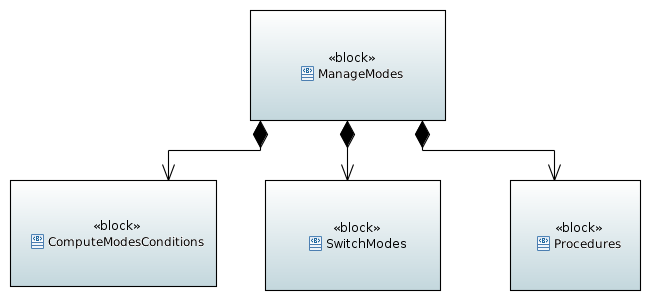
\includegraphics[scale=1]{../SysML/FunctionalArchi_Modes.png}
\caption{Modes subfubction architecture}
\end{figure}
\end{landscape}

Three subfunctions are defined:
\begin{description}
\item[ComputeCondition] specifies the conditions to define a mode transition according condition table of section 4.6.3 of \citep{subset-026}
\item[SwitchModes] performs the mode selection according the conditions and priorities defined in transition table  section 4.6.2 of \citep{subset-026}
\item[Procedures] performs all specific procedure linked to mode management and defined in  \citep{subset-026} sections 5.4, 5.5, 5.6, 5.7, 5.8, 5.9, 5.11, 5.12, 5.13, 5.19.
\end{description}


See below section "Detailled model" for details.

\begin{landscape}
\begin{figure}[hbtp]
\centering
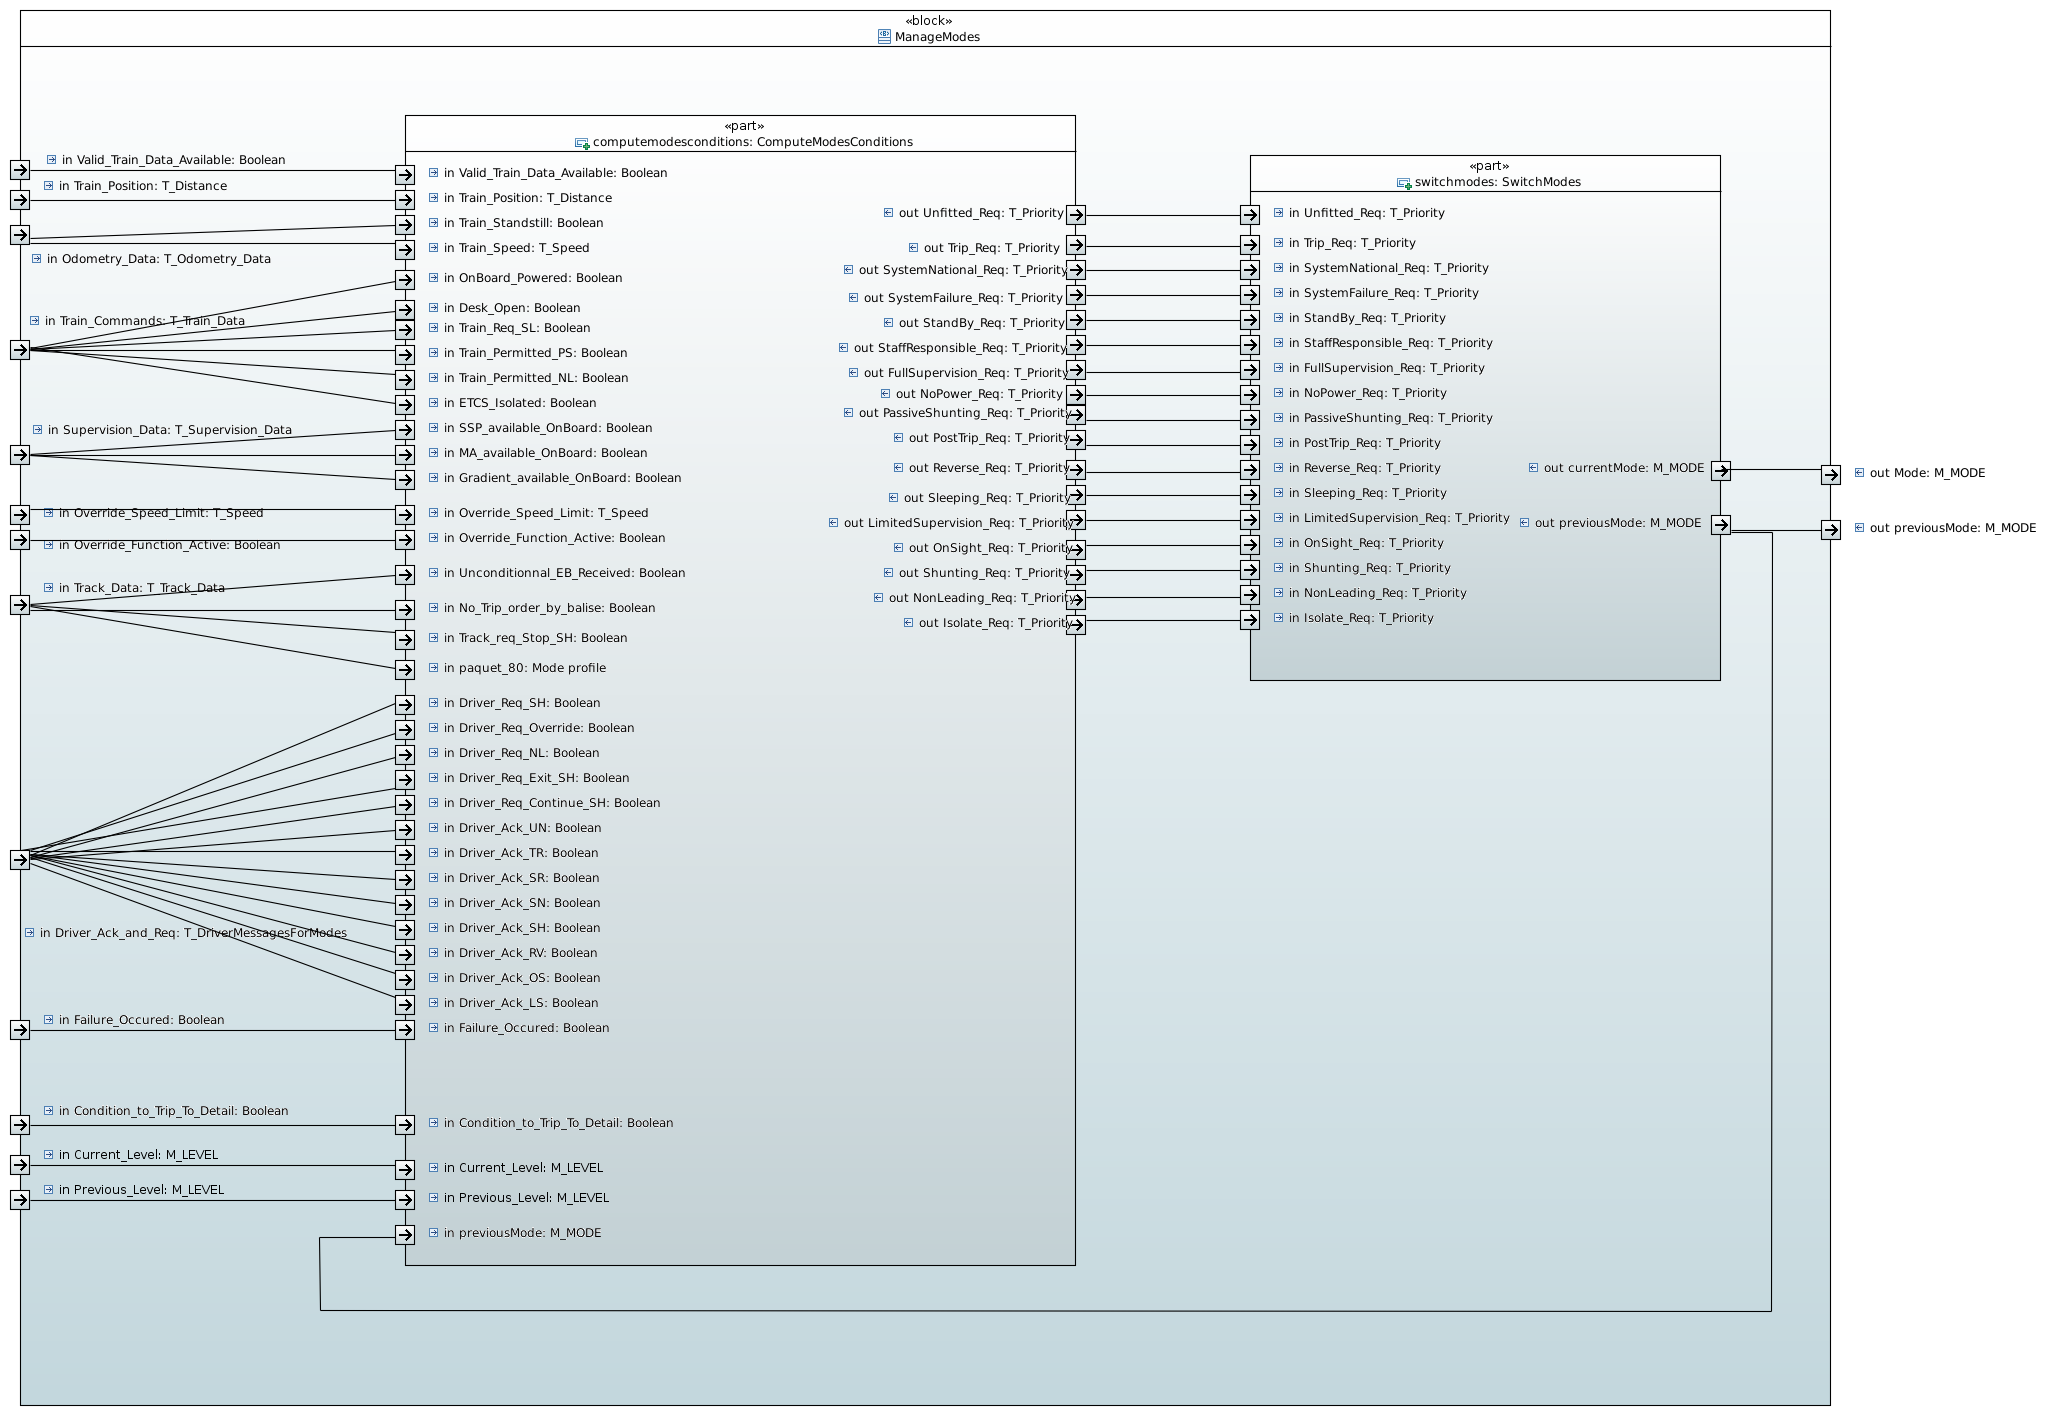
\includegraphics[scale=0.45]{../SysML/ManageModes.png}
\caption{Modes subfunction dataflow}
\end{figure}
\end{landscape}

\section{Interface}

\subsection{Public Types of Modes}


\begin{center}


\renewcommand{\arraystretch}{2} 
\tablehead{%
\hline
\rowcolor{gray} 
Name & Type &  Comments  \\ 
\hline}
\tablefirsthead{
\hline
\rowcolor{gray} 
Name & Type &  Comments  \\ 
\hline 
}
\begin{supertabular}{| m{3cm} | m{6cm} | m{4cm} |}
\hline 
T\_Cab	& enum \{A, B, unknown\}	& Assumption : Train has exactly two cabins see \citep{subset-034} \\ 
\hline
T\_Level & 	enum \{L0, L1, L2, L3, LNTC\}	& \textcolor{blue}{To check with level section}  \\ 
\hline
T\_Mode	& enum \{NP, SB, PS, SH, FS, LS, SR, OS, SL, NL, UN, TR, PT, SF, IS, SN, RV\}	& M\_MODE can not be used: No power mode is not defined. \\ 
\hline
T\_MA	& enum \{Profile\_OS, Profile\_LS, Profile\_SH, No\_Profile\}	& M\_MAMODE can not be used: No Profile is not defined. \\ 
\hline
T\_Mode\_Profile & 	Structure \{Distance : int, Mode :  T\_MA, Speed : int, Length : int, Length\_Ack : int \}	 & \textcolor{red}{To check with filtering function and internal structure.}  \\ 
\hline 
\end{supertabular} 


\end{center}

\subsection{Inputs of ManageModes}


\begin{center}

\tablehead{%
\hline
\rowcolor{gray} 
Name & Type & Consummers & Comments  \\ 
\hline}
\tablefirsthead{
\hline
\rowcolor{gray} 
Name & Type & Consummers & Comments  \\ 
\hline 
}
\begin{supertabular}{| m{6cm} | m{3cm} | m{3cm} | m{3cm} |}
\hline 
Ack\_Req\_LS\_Display  & bool & To Dmi & procedure ?  \\ 
\hline 
Ack\_Req\_OS\_Display  & bool & To Dmi & procedure ?  \\ 
\hline  
Ack\_Req\_SH\_Display  & bool & To Dmi & procedure ?  \\ 
\hline 
Ack\_Req\_SN\_Display & bool & To Dmi & procedure ?  \\ 
\hline 
Ack\_Req\_SR\_Display & bool & To Dmi & procedure ?  \\ 
\hline 
Ack\_Req\_UN\_Display & bool & To Dmi & procedure ?  \\ 
\hline 
Cab &	T\_Cab	& From TIU &  \\ 
\hline 
ConditionToTrip & bool & To clarify& • \\ 
\hline 
Continue\_Shunting\_Function\_Active & bool &  Procedure ?& • \\ 
\hline 
CurrenT\_Level	& T\_Level	& Internal from Level Management& • \\ 
\hline 
Desk\_A\_Open & bool & From TIU & • \\ 
\hline 
Desk\_B\_Open & bool & From TIU & • \\ 
\hline 
Driver\_Ack\_LS & bool & From DMI & procedure ?  \\ 
\hline 
Driver\_Ack\_OS & bool & From DMI & procedure ?  \\ 
\hline 
Driver\_Ack\_RV & bool & From DMI & procedure ?  \\ 
\hline 
Driver\_Ack\_SH & bool & From DMI & procedure ?  \\ 
\hline 
Driver\_Ack\_SN & bool & From DMI & procedure ?  \\ 
\hline 
Driver\_Ack\_SR & bool & From DMI & procedure ?  \\ 
\hline 
Driver\_Ack\_TR & bool & From DMI & procedure ?  \\ 
\hline 
Driver\_Ack\_UN & bool & From DMI & procedure ?  \\ 
\hline 
Driver\_Req\_ExiT\_SH & bool & From DMI & procedure ?  \\ 
\hline 
Driver\_Req\_NL & bool & From DMI & procedure ?  \\ 
\hline 
Driver\_Req\_Override & bool & From DMI & procedure ?  \\ 
\hline 
Driver\_Req\_SH & bool & From DMI & procedure ?  \\ 
\hline 
Emergency\_Stop\_Message\_Received & bool & From Balises ?& • \\ 
\hline 
Estimated\_Front & int & Train position ?& • \\ 
\hline 
ETCS\_Isolated & bool & From TIU& • \\ 
\hline 
Failure\_Occured & bool & Internal ?& • \\ 
\hline 
Previous\_Level & 	T\_Level	& Internal from Level Management& • \\ 
\hline 
MA\_SSP\_Gradiant\_Available & bool & From supervision ?& • \\ 
\hline 
Max\_Safe\_Front & bool & Train position ?& • \\ 
\hline 
Mode\_Profile\_On\_Board &	T\_Mode\_Profile &	Stored from  packet 80 & • \\ 
\hline 
No\_Trip\_Order\_Given\_By\_Balise & bool & From Balises ?& • \\ 
\hline 
OnBoard\_Powered & bool & From TIU& • \\ 
\hline 
Override\_Function\_Active & bool & Procedure ?& • \\ 
\hline 
Shunting\_Granted\_By\_RBC & bool & Radio ?& • \\ 
\hline 
Stop\_Shunting\_Stored & bool & Procedure ?& • \\ 
\hline 
Train\_Permitted\_NL & bool & From TIU& • \\ 
\hline 
Train\_Permitted\_PS & bool & From TIU & • \\ 
\hline 
Train\_Req\_SL & bool & From TIU& • \\ 
\hline 
Train\_Speed\_Under\_Override\_Limit & bool & From supervision ?& • \\ 
\hline 
Train\_Standstill & bool & From supervision ?& • \\ 
\hline 
Train\_Speed & int & From supervision ?& • \\ 
\hline 
Valid\_Train\_Data\_Stored & bool & Internal ?& • \\ 
\hline 
\end{supertabular} 

\end{center}

\subsection{Outputs of ManageModes}

\begin{center}

\tablehead{%
\hline
\rowcolor{gray} 
Name & Type & Consummers & Comments  \\ 
\hline}
\tablefirsthead{
\hline
\rowcolor{gray} 
Name & Type & Consummers & Comments  \\ 
\hline 
}
\begin{supertabular}{| m{6cm} | m{3cm} | m{3cm} | m{3cm} |}
\hline 
currentMode & T\_Mode & • & • \\ 
\hline 
previousMode & T\_Mode & • & • \\ 
\hline 
\end{supertabular} 
	


\end{center}


\section{Requirements}

\section{Detailled model - SCADE}

\subsection{ComputeModesConditions subfunction}

\subsection{SwitchModes subfunction}


\subsection{Procedures subfunction}

% end of chapter